
%% !TEX root = manual.tex

\section{Fixed-Time Quanta Charts}

\label{sec:tutorials:ftq}

\begin{figure}[h!]
\centering
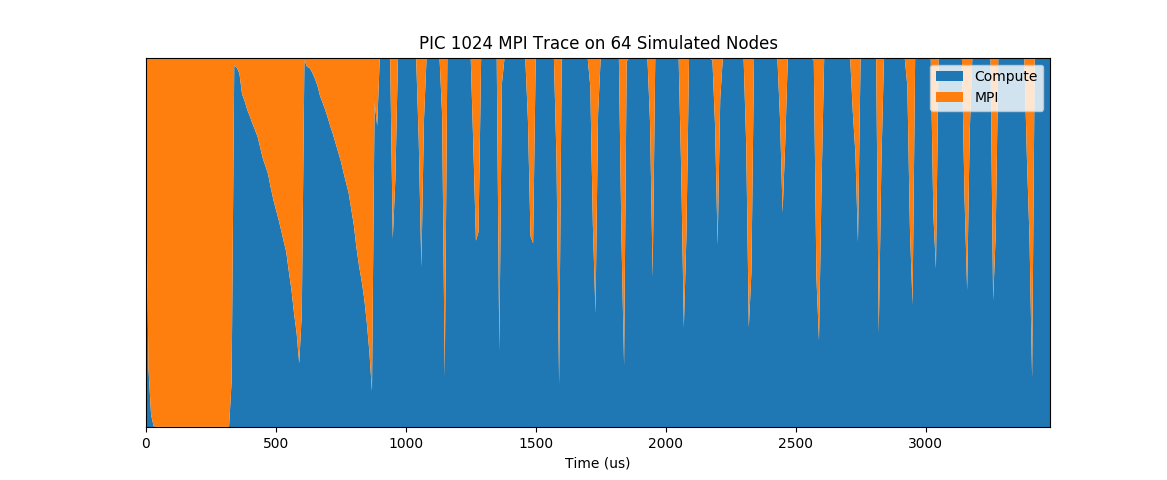
\includegraphics[width=0.6\textwidth]{figures/matplotlib/ftq/pic1024.png}
\caption{Application Activity (Fixed-Time Quanta; FTQ) histogram}
\label{fig:ftq}
\end{figure}

Another way of visualizing application activity is a fixed-time quanta (FTQ) chart.
While the call graph gives a very detailed profile of what critical code regions, they lack temporal information. 
Figure \ref{fig:ftq} displays the proportion of time spent by ranks in MPI communication and computation in a PIC trace replay with respect to simulation time.
After running, two new files appear in the folder: \inlineshell{<fileroot>_app1.py} and \inlineshell{<fileroot>_app1.dat} that can use Python's matplotlib to generate plots.
Previously, plots were generated using Gnuplot, but this has been deprecated in favor of much more aesthetically pleasing maplotlib output.

\begin{ShellCmd}
your_project # python output_app1.py --help
usage: output_app1.py [-h] [--show] [--title TITLE] [--eps] [--pdf] [--png]
                      [--svg]

optional arguments:
  -h, --help     show this help message and exit
  --show         display the plot on screen
  --title TITLE  set the title
  --eps          output .eps file
  --pdf          output .pdf file
  --png          output .png file
  --svg          output .svg file
\end{ShellCmd}

Generating the histogram requires matplotlib, and visualizing the histogram interactively with \inlineshell{--show} requires a screen or X11 forwarding.
FTQ aggregates tags into tunable time "epochs".
An epoch states the ratio of each tag represented at a point in time.
Larger epochs will smooth the graph and decrease the quantity of data required to render a plot; while a smaller epoc will add more detail, at the risk of making the plot excessively volatile.


SST/macro activates FTQ for a given application as:

\begin{ViFile}
node {
 app1 {
  name = sstmac_mpi_testall
  launch_cmd = aprun -n 8 -N 2
  ftq {
   type = ftq_calendar
   epoch_length = 1ms
   output = ftq
   group = app1
  }
  print_times = false
  message_size = 400B
 }
}
\end{ViFile}
where the \inlinefile{fileroot} a path and a file name prefix.
